\vspace{\baselineskip}
\vspace{\baselineskip}

\section{Controles}
El juego usa un sistema de control por teclado y ratón. Mediante clicks derechos del ratón se mueve al personaje por el mapa. Si se cliquea sobre un enemigo, el personaje aplicará un ataque básico sobre este.
Las teclas Q W E activan las tres habilidades básicas y la tecla R la habilidad definitiva.

\vspace{\baselineskip}

La cámara del jugador tiene dos modos: \emph{auto} y \emph{manual}. En modo \emph{auto}, la cámara sigue el movimiento del jugador y siempre está centrada sobre este. En modo \emph{manual}, la cámara está fija y no sigue al jugador. En este modo, la cámara se desplaza arrastrando el ratón hacia los bordes de la pantalla. Al pulsar la tecla \emph{Space}, se cambia entre un modo y otro.

\vspace{\baselineskip}

\begin{figure}[h]
	\centering
	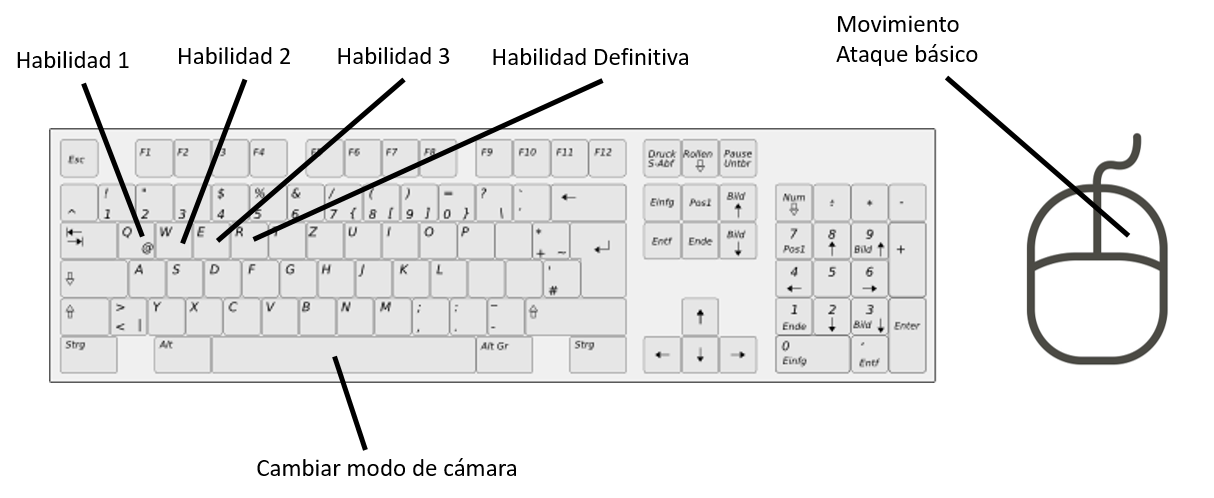
\includegraphics[width=0.8\linewidth]{figures/controles.png}
	% \caption{Controles}
\end{figure}

% ==============================================================================

\newpage

\subsection{Sistema visual}

Durante el desarrollo de las partidas el HUD se compone de 2 partes:

\vspace{\baselineskip}

\subsubsection{Player HUD}
Situado en la parte inferior de la pantalla, incluye la vida del personaje y las habilidades, con su respectivo cooldown e información adicional (casteo, si está activa, etc.).

\begin{figure}[h]
	\centering
	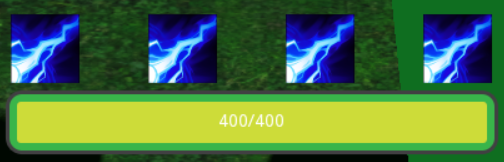
\includegraphics[width=0.6\linewidth]{figures/PlayerHUD}
	% \caption{Habilidades del personaje y barra de vida.}
	\label{fig:PlayerHUD}
\end{figure}

\vspace{\baselineskip}

\subsubsection{Match details}

En la parte superior de la pantalla se muestra el estado actual de los objetivos de la partida. La información mostrada variará según el modo del juego:

\begin{itemize}
	\item \textbf{Deathmatch}: Muestra el número de vidas restantes de cada equipo.
	\item \textbf{Captura}: Muestra la puntuación de cada equipo así como el tiempo de partida restante.
\end{itemize}

\begin{figure}[h]
	\centering
	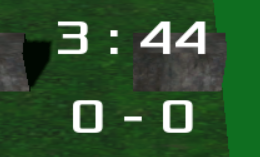
\includegraphics[width=0.6\linewidth]{figures/MatchDetails}
	% \caption{Match Details del modo de juego \emph{Captura}.}
	\label{fig:MatchDetails}
\end{figure}
